\documentclass[11pt,letter]{article}
\usepackage[left=2cm, right=3cm, top=2cm, bottom=2cm]{geometry}
\usepackage{amsmath, amsthm, enumitem, graphicx, tabularx, multirow, amssymb, array, afterpage,csquotes}
\usepackage{natbib}
\usepackage{setspace}
\setlength{\parskip}{0.1cm}
\usepackage[english]{babel}
\usepackage{floatpag}
\setlength{\parindent}{0.0in}
\setlength{\parskip}{\baselineskip}
\setenumerate{leftmargin=2cm, nolistsep}
\setitemize{leftmargin=3cm, nolistsep}
\newcommand{\sbt}{\,\begin{picture}(-0.4,2.5)(-0.4,-2.5)\circle*{2}\end{picture}\ }

\begin{document}
\pagenumbering{arabic}
\setcounter{page}{1}
\thispagestyle{plain}
\noindent Consider the irrigation problem by Lagrangian of Section 3.3:

This is an equation with automatic numbering :
\begin{equation}\label{eq:3DynLag} 
\mathbb{L} = \sum_{t=0}^{\infty}\rho^t\{ax_t - (b/2)x_t^2 - (c/2)u_t^2 + \rho \lambda_{t+1}[(1 - d)x_t + u_t - x_{t+1}]\}.
\end{equation}  

I refer to this last equation by its automatic number as Equation \ref{eq:3DynLag}.

Placing an asterisk does not number an equation
\begin{equation*} 
 x_{t+1}=abc
\end{equation*}  


This similarly produces a display equation without a number
$$ x_{t+1}=abcefg$$

This similarly produces an inline equation $ x_{t+1}=abcefg$ (never has a number)

This is bunch of equations in the same block that are counted, but tagged my way   
The FOCs are 
\begin{align}\label{eq:3DynLagFOC1}\tag{FOC1}
\begin{split} 
\partial\mathbb{L}/\partial u_t &= \rho^t\{-cu_t + \rho\lambda_{t+1}\} = 0 \\
\Rightarrow u_t &= \rho\lambda_{t+1}/c
\end{split} 
\end{align}
\begin{align}\label{eq:3DynLagFOC2}\tag{FOC2}
\begin{split}
\partial\mathbb{L}/\partial x_t &= \rho^t\{a - bx_t + (1 - d) \rho\lambda_{t+1}\} - \rho^t\lambda_t = 0 \\
\Rightarrow \lambda_t &= a - bx_t + (1 - d)\rho\lambda_{t+1}
\end{split} 
\end{align}
\begin{align}\label{eq:3DynLagFOC3}\tag{FOC3}
\begin{split}
\partial\mathbb{L}/\partial [\rho\lambda_{t+1}] &= \rho^t\{(1 - d)x_t + u_t - x_{t+1}\} = 0 \\
\Rightarrow x_{t+1} &= u_t + (1 - d)x_t +  
\end{split} 
\end{align}

This is regular text with inline equations in $(x_t, u_t)$.

Nothing special is required to reference a numbered but specially tagged Equation like  \ref{eq:3DynLagFOC3} .

This is how you do easy enumerations with capital letter and parentheses for labels. The default is arabic*. The indentation was defined in the header but you can modify other parameters as well, either locally or globally (i.e. in the header) 

\begin{enumerate}[label=(\Alph*)]\itemsep0pt \parskip0pt \parsep0pt
	\item first item 
	\item second item 
	\item third item
\end{enumerate}

This is how you do easy bullet lists
\begin{itemize}
	\item first item 
	\item second item 
	\item third item
\end{itemize}


Here are matrices
\begin{equation*}
 \begin{bmatrix} u_{t+1} \\ x_{t+1} \end{bmatrix} = \begin{bmatrix} {{\frac{c+ b \rho}{(1-d) \rho c}}}&{{\frac{b}{c}}} \\ 
  {{1}}&{{(1-d)}}  \end{bmatrix} \begin{bmatrix} u_t \\ x_t \end{bmatrix} + \begin{bmatrix} - \frac{a}{c(1-d)} \\ 0 \end{bmatrix} 
\end{equation*}

I include Figure \ref{fig:myfirstpic} because it is very useful.\footnote{You place the text of a footnote midtext, exactly where you want the reference to it.}

\begin{figure}[htbp]
	\centering
		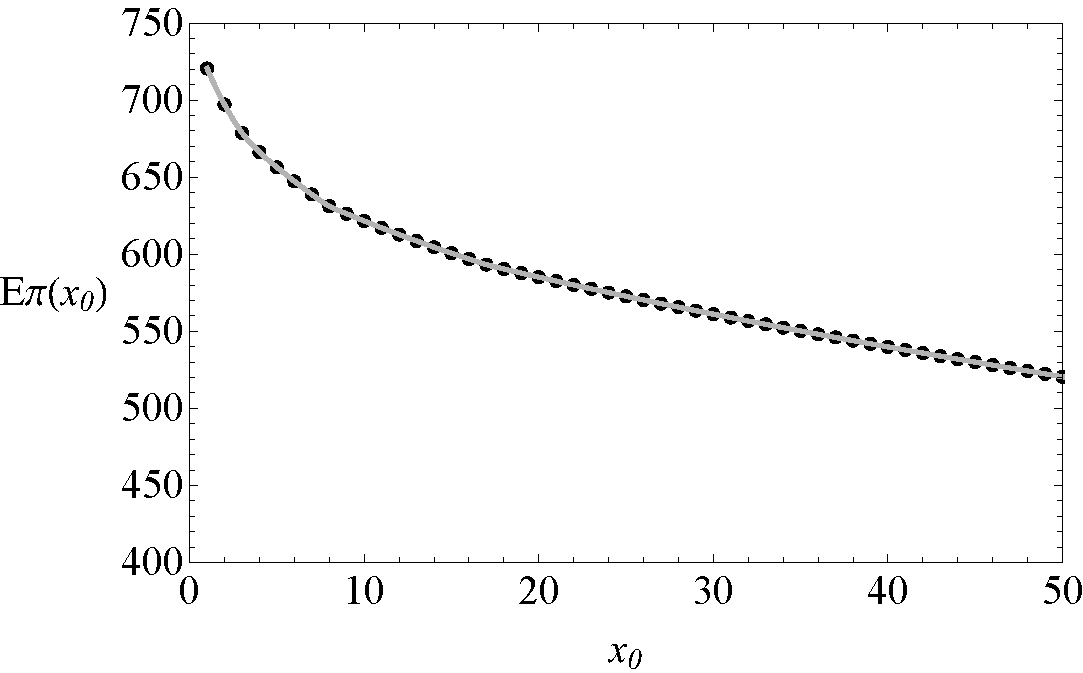
\includegraphics[width=0.80\textwidth]{Pest3PeriodV0spline.pdf}
	\caption{The very useful graph}
	\label{fig:myfirstpic}
\end{figure}

Controlling the placement of figures can be a bit of a pain! I most often use [!h] as the option as it tends to place the figure closest to where it is coded.

\% comments out a line in the code. 

% a comment 



This is a Table

\begin{table}[h]
\centering  
\caption{Adjustment of Round 1 to Round 2 Offers for Subjects Choosing Incorrectly in BDM1}  \small
\label{exposedBDM1}
\begin{tabular}{lcc}\hline
                               &               Exposed to Round 1 Error & Not Exposed to Round 1 Error              \\ \hline 
                              
Total Subjects           & 41 (100\%)                   & 109 (100\%) \\
Move onto optimum (\$2)  & 3 (7.3\%)                    & 8 (7.3\%)   \\
Move Toward Optimum      & 25 (61.0\%)                  & 35 (32.1\%) \\
Choose same offer ratio  & 7 (17.1\%)                   & 25 (22.9\%) \\
Move away from optimum   & 6 (14.6\%)                   & 41 (37.6\%) \\ \hline
\end{tabular}
\end{table}


For references, all of this is due to \citet{simsetal2016}. There are different ways of citing depending on what you need in your text:

\citet{simsetal2016}

\citep{simsetal2016}, do cool shit.

\citeauthor{simsetal2016} are cool dudes

The bibliography follows. It needs a database called myref that you populate as well as a bibliography style file. Here, the style is wsc and the required file is wsc.bst


\newpage


%%%%%%%%%%%%%%%%%%%%%%%%%%%%%%
\bibliography{myref}
\bibliographystyle{wsc}


 



\end{document}